\chapter{Implementáció}

\section{Szerverek}

\subsubsection{Safranek}

\paragraph{}
A feladatok közül a legelső a már meglévő Safranek szerver frissítése és konfigurálása volt. 
A Safraneken egy Ubuntu server 16.04-es verzió futott, így nem volt szükség sem az operációs rendszer, sem pedig a disztribúció cseréjére, mivel a projektet az Ubuntu szerver ezen verziója tökéletesen kiszolgálja.
A frissítéseket követően, a Jenkins CI futtatását kellett előkészíteni. 
Egy jenkins nevű felhasználót kellett létrehozni, hogy szeparáltan lehessen futtatni a programokat és az autentikáció során ne a root felhasználó adatait keljen felhasználni. 

Mivel a TomCat és a Jenkins is egy-egy java alapú alkalmazás ezért a Java JRE és JDK legfrissebb verzióját kellett felkellet telepíteni. 
Azt a következő két parancs alkalmazásával: 

----"sudo apt-get install default-jre \&\& sudo apt-get install default-jdk"------

A Jenkins CI-t szervletként futtatható verziójához telepíteni kellett az Apache TomCat-ot. 
A TomCat 8.5.8-as verziója volt a legfrissebb, így ezt a verzió került fel a Safranekre. 
A jenkins felhasználó "home" könyvtárában került elhelyezésre egy "tomcat" nevű mappába. 
Mielőtt a jenkins felhasználóval elindult volna a TomCat a "~/tomcat/conf/tomcat-users.xml" fájlt a \ref{fig:tomcatxml} ábrán láthatóan kellet módosítani, hogy a webes menedzment elérhető legyen. 
Ezt a Nano szövegszerkesztő segítségével lehetett elvégezni. 

\begin{figure}[h]
	\centering
	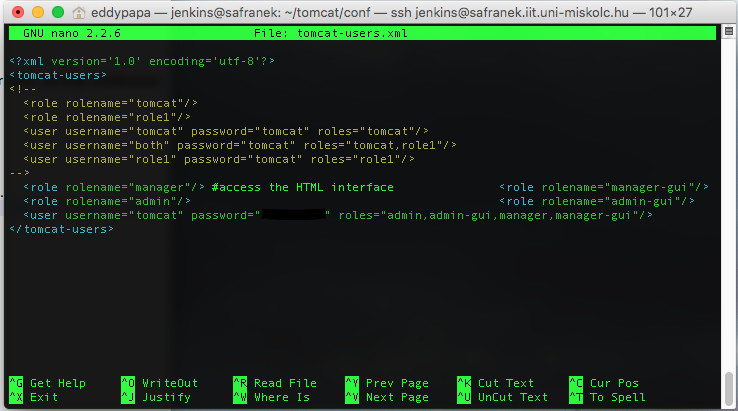
\includegraphics[width=1\linewidth]{pics/tomcatxml}
	\caption{TomCat felhasználó beállítása}
	\label{fig:tomcatxml}
\end{figure}

\paragraph{}
Következhetett a Jenkins CI telepítése. A Jenkins CI legfrissebb verziója a 2.32.2 volt. 
A letöltött "jenkins.war" fájlt a "~/tomcat/webapps mappába kellett letölteni. 
A letöltés befejeztével elindíthatóvá vált a TomCat. 
Ezt a "~/tomcat/conf" mappában található "startup.sh" scripttel kellett megtenni. 
A http://safranek.iit.uni-miskolc.hu:8080/jenkins webcímen elérhetővé is vállt a Jenkins CI.

\begin{figure}[h]
	\centering
	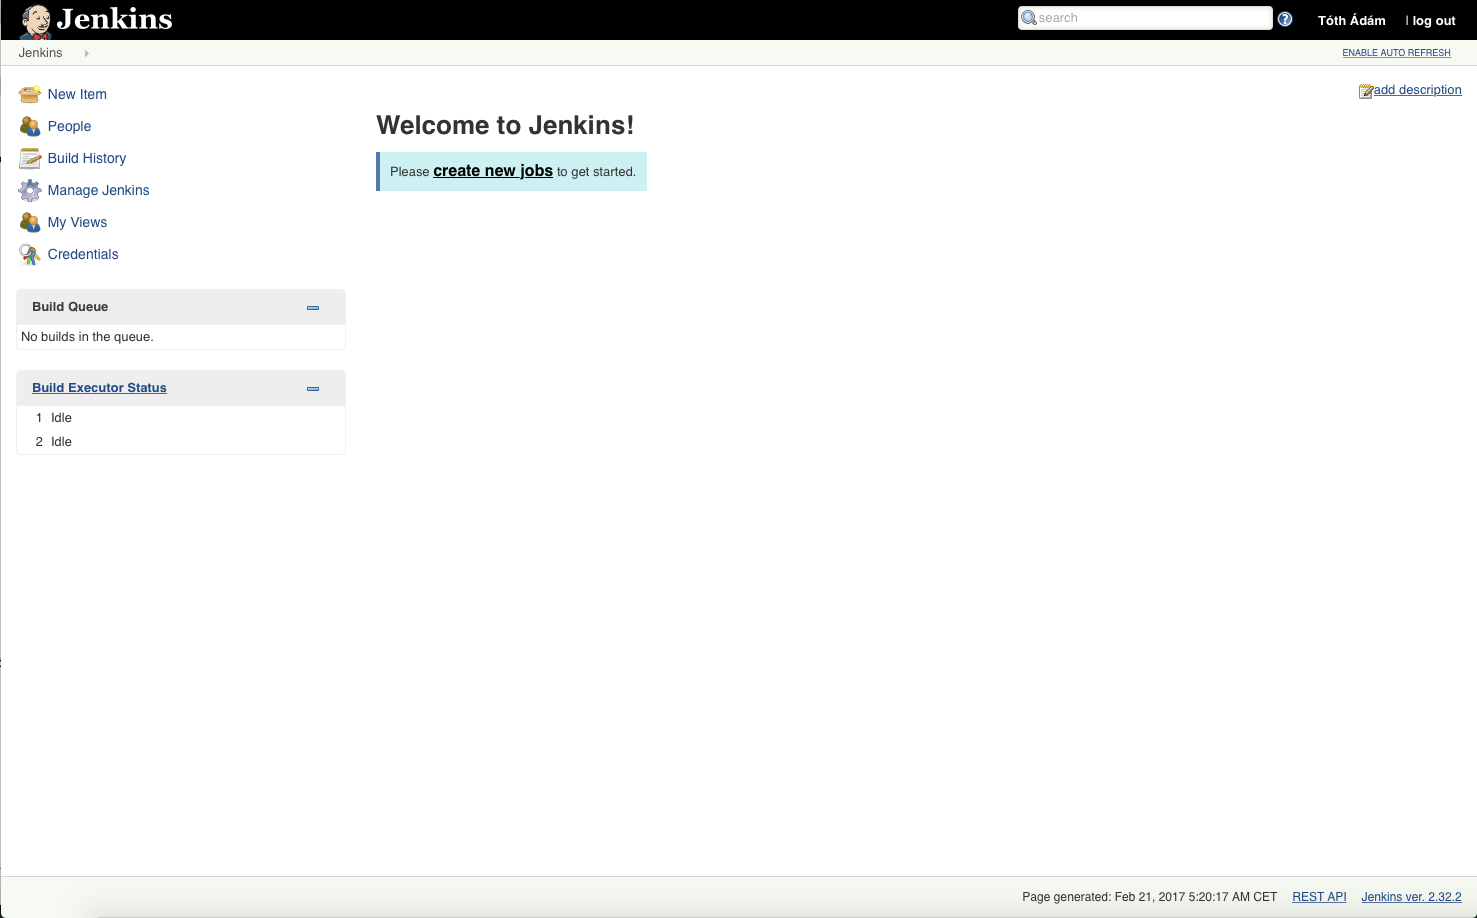
\includegraphics[width=1\linewidth]{pics/clearjenkins}
	\caption{Első belépés a Jenkins CI felületére}
	\label{fig:clearjenkins}
\end{figure}

\paragraph{}
Az első felhasználó létrehozásához és a komponensek telepítése előtt egy a "/.jenkins/secrets/initialAdminPassword" fájlban található jelszót kell bemásolni a formba a folytatáshoz. 
Miután ez megtörtént a Jenkins CI admin felülete tárul elénk \ref{fig:clearjenkins}. 

\subparagraph{Jenkins}

A Jenkin CI 


